\chapter{Äristrateegia}
\section{Strateegia olemus}
Äritrateegiast on kõikvõimalikes vormides kirjutatud palju kuid siiski ei ole tegu valdkonnaga, kus eksisteeriks selgelt domineeriv mõttsuund. Ka strateegia enese definitsioon ei ole üheselt paigas ning seega onn paljul tavapäraselt strateegiaks peetul strateegia enesega vähe pistmist\cite{de2006strategy}. Freedman\index{Freedman, Lawrence} ütleb, et see peabki nii olema, sest ta strateegia tegeleb valikutega ning aruteluga nende üle. Valikud ise aga tuginevad laiale spektrile diskursustele.\cite{freedman2013strategy} 

Kuidas ka ei ole, \citeauthor{de2006strategy, rumelt1991strategic} toovad rea põhiküsimusi\cite{rumelt1991strategic}, millega äristrateegia selle ühel või teisel moel tegeleb:
\begin{description}\index{Strateegia!Põhiküsimused}
	\item[Eesmärgid] Mis suunas organisatsioon liigub ning, seeläbi ka vältimatult, mis suunas ta \emph{ei} liigu
	\item[Positsioon] Milline positsioon turul annab organisatsioonile suurima konkurentsieelise, olgu siis läbi olemasolevate resusrsside või turusituatsiooni. Turupositsiooni mõiste on samuti lai, kuid peamine on, et strateegia tegeleb organisatsiooni paigutamisega suhtes teiste turuosalistega. Näiteks on strateegiline küsimus, kas tegeleme pigem haljastusse või pensionäride tillukestesse aedadesse sobivate muruniidukitega.
	\item[Pakutavad tooted ja teenused] Millises sektoris organisatsioon osaleb ning milliseid teenuseid ja tooteid pakub. Kui eelmine küsimus oli seotud turuga, siis siin me saame näiteks küsida, kas me pigem tegeleme muruniidukite tootmise, hoolduse või näiteks laenutamisega
	\item[Tegevusulatus ja mitmekesisus] Kui suurt mitmekesisust pakutavates toodetes ja teenustes ning organisatsiooni tegevuses laiemalt talutakse ning kui suurt osa võimalikust toodete/teenuste spektrist kaetakse
	\item[Ressursside suunamine] Kuhu me kulutame oma piiratud ressursid. Tegemist on teatud mõttes juhtimisliku põhiküsimusega keerulise komplekti piiratud vahendite kulutamisest võimalikult kasulikul moel. Kuigi strateegia ei saa anda siin täpset vastust, peab ta vastuse leidmist toetama. Strateegia ei ütle, mitu inimest tegeleb müügi ja mitu klienditeenindusega kuid ta võib öelda, et meie jaoks on müük olulisim ning klienditeenindus pole oluline
	\item[Organisatsiooni disain] Milline on organisatsiooni struktuur, millised poliitikad kehtivad ning milliseid administratiivseid vahendeid kasutatakse. Ehk, kuidas organisatsioon määratleb ja koordineerib tööd
\end{description}


Siinkohal võib tekkida küsimus, kus nende küsimustega igapäevane tegelemine muutub taktikast strateegiaks. Freedman ütleb, et tegelikult on vahe strateegia ja taktika vahel seotud vaid organisatsiooni hierarhia ning vähemal määral otsuste mõju ning ajahorisondiga. Kuid mõlemal juhul on otsuste taga samad printsiibid. 
\begin{marginfigure}
	\begin{center}
		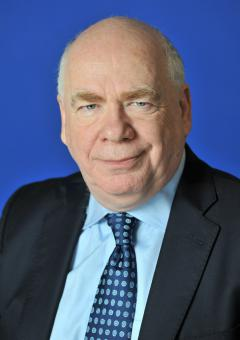
\includegraphics[width=.84\linewidth]{freedman.jpg}
		\caption{Lawrence Freedman}
		\label{fig:freedman}
	\end{center}
\end{marginfigure}

Üsna levinud on kontseptsioon \enquote{strateegilisest plaanist}\index{Strateegia!Plaan}. Ehk arusaam, et strateegia seab eesmärgid ning sammud nendeni jõudmiseks. Nii mõtlevad tihti insenerid: meil on lahendamist vajav probleem, me töötame välja plaani ja viime selle ellu. Meil on vaja kuule jõuda ning sinna me ka jõuame. Konks on selles, et kuu ei ürita raketi ehitamise käigus aktiivselt eest ära joosta. Nii arutledes on raske mitte nõustuda Freedmaniga, kes ei pea õigeks mõelda strateegiast kui plaanist\sidenote{Ta tsiteerib Mike Tysonit\index{Tyson, Mike}: \enquote{Everyone has a plan 'till they they get punched in the mouth}}. Tema argumentatsioonis tugineb strateegia alati organisatsiooni positsioonile ning positsiooni muutudes muutub ka strateegia, eesmärgid ja plaan. Strateegia praktiline iva ei ole Freedmani järgi mitte mingi konkreetse eesmärgi saavutamine vaid jõudmine praegusest paremasse positsiooni. Samuti ei lõpe miski eesmärkide saavutamisega. Revolutsioonile järgneb vajadus valitseda, konkurendi üle võtmisele vajadus ühist organisatsiooni ehitada\sidenote{\enquote{Strategy is not a three-act play. It's a soap opera}}. 


Milline siis on Freedmani konstruktiivne vaade strateegiale? Tema käsitluses on strateegia aluseks soov kontrollida tulevikku suuremal määral, kui konkurendid. Tuleviku ennustamise aluseks on aga mõttemudel. Mõttemudeli mõistet seletab ehk kõige paremini Hawking\cite{mlodinow2010grand}. Ta väidab, et me tajume maailma alati läbi mudeli ning et selle mudeli peamiseks omaduseks on tema ennustusväärtus: kui täpselt suudab mudel mineviku alusel ennustada tulevikku. \sidenote{Hea mõttemudel ei ole siiski tingimata seotud isikliku heaoluga. Giordano Bruno mudel oli valitsevast maailmakäsitlusest oluliselt parema ennustusväärtusega}. 

Seega muutub strateegias põhimõtteliseks küsimuseks sobiliku mõttemudeli loomine, praeguse olukorra mõtestamine organisatsiooni soovitud suunas liigutada aitaval viisil. Kuid organisatsioon ei koosne ainult juhist ning seega on strateegia puhul oluline, et organisatsiooni liikmed võtaksid omaks just juhi loodud malli ning suudaksid ja tahaksid seda ka tegutesse valada. See on juhi töö, mille aluseks on teatud empaatiavõime. Ei ole mõeldav asendada üht mõttemudelit teisega toda esimest esmalt mõistmata. Üheks viisiks tagada mõttemudeli jagatust on kaasata organisatsioon selle koostamisse. Tuleb nõustuda Eisenhoweriga\index{Eisenhower, Dwight D.}, kes ütles \quote{\enquote{Plans are worthless, but planning is everything}}. 

Kuigi strateegiat ei ole mõistlik vaadata liikumisega konkreetse eesmärgi poole, on strateegia kui teema mõistmiseks oluline mõista organisatsioonide liikumapanevaid jõude. \citeauthor{de2006strategy} sõnastab selle nii:

\begin{center}
	\textbf{Väärtuse loomine omanikele ning teistele osapooltele läbi kliendile väärtuse pakkumise}
\end{center}

On oluline mõista, et \enquote{väärtus}\index{Väärtus} võib tähendada oluliselt laiemat mõistete skaalat, kui lihtsalt finantstulu. Väärtust reeglina \emph{mõõdetakse} rahas kuid ta ei pruugi \emph{olla} rahaline. Nii mõnigi pillimees peab muusikastuudiot mitte sellest omanikutulu teenimiseks kui omamaks võimalust igal hetkel koos sõpradega oma hobiga tegeleda. Ehk, väärtus on oma olemuselt subjektiivne. 

Siit näeme, et organisatsiooni liikumissuund on sõltuv omanikest ning \enquote{teistest osapooltest}. Kui omaniku mõiste on reeglina juriidiliselt täpselt määratletud, siis teiste osapoolte määratlus on segasem\sidenote{Ja, globaalses kontekstis, järjest segasemaks läheb. Vt. \nameref{sec:architecture:paradigm}}. 

Oleme näinud, et strateegia on oma olemuselt dünaamiline nähtus. Teda suunavad vähemalt kolm võtmefaktorit:
\begin{itemize}
	\item Strateegia ise läbi organisatsiooni positsiooni ning seega ka strateegia nihutamise
	\item Organisatisooni omanike\index{Omanik} ja arvesse võetavate \enquote{teiste osapoolte} ringi muutused
	\item Omanike ja teiste osapoolte arusaam väärtusest\sidenote{Eriti keeruline strateegiline olukord tekib, kui omanike ja muude huvigruppide arusaam väärtusest aeglaselt lahku triivivad}
\end{itemize}
\begin{marginfigure}
	\begin{center}
		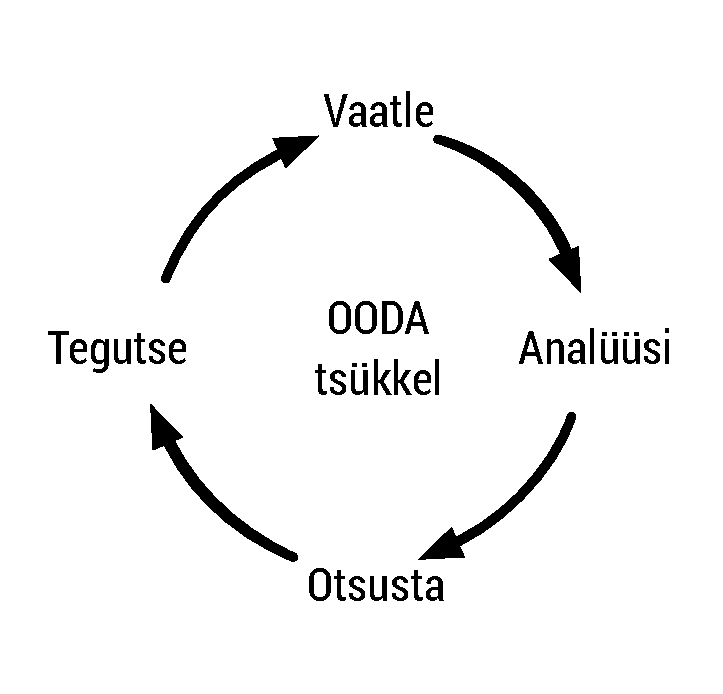
\includegraphics[width=\linewidth]{ooda.pdf}
		\caption{OODA/VAOT tsükkel}
		\label{fig:ooda}
	\end{center}
\end{marginfigure}

Strateegiast kui dünaamilisest nähtusest aitab ehk mõelda VAOT\sidenote{Originaalis \emph{OODA. Observation, Orientation, Decision, Action}} tsükkel, mille autoriks on John Boyd\index{Boyd, John}. Boyd oli inseneritaustaga lendur ja militaarteoreetik kelle karjäärist paistab harvanähtav võimekus tegeleda probleemidega väga laial abstraktsiooniastmete skaalal. Oma kogemusest lahinglendurina suutis ta sünteesida mõjukaid teooriaid, neid populariseerida ning suunata ka nende  rakendamist. Tema VAOT tsükkel koosneb järgmistest, järjest korduvatest, sammudest:

\begin{description}
	\item[Vaatle] Kogu andmeid olukorra kohta
	\item[Analüüsi] Analüüsi ja sünteesi kogutud andmeid lähtudes oma hetkepositsioonist ja mõttemudelist
	\item[Otsusta] Määra, jällegi tuginedes oma mõttemudelile, kindlaks tegutsemissuund
	\item[Tegutse] Vii otsused ellu
\end{description}


Boyd'i idee seisnes selles, et võitmiseks\sidenote{Freedman osundab, et võit on strateegilises mõtlemises liigselt rõhutatud. Tõpeoolest, Napoleoni strateegia tugines suuresti otsustavale võidule kuid ka tema 1812. aasta sõjakäik näitas, et see ei ole alati võimalik. Tänapäevases tehnoloogiliselt keerulises olukorras on nii militaarselt kui äriliselt üha raskem vastast otsustava löögiga põlvili sundida. Strateegia oluliseks komponendiks on võimekus oodata, koalitsioone moodustada ja mitte kohe rünnata.} tuleb luua olukordi, kus ollakse suuteline vastasest kiiremini õigeid otsuseid tegema. Nii ei ole teisel osapoolel võimalik õigesti käituda: olukord muutub enne, kui te reageerida jõuab. Sellest ka keskendumine otsustusprotsessile ning adapteerumisele mitte ühele konkreetsele olukorrale vaid muutuvale situatsioonile üldiselt.

\section{Strateegiamõtte ajaloost}
Strateegia mõiste sellisena, nagu me teda täna tunneme, kerkis esile militaarvaldkonnas 18. sajandil. Sõna \emph{stratagos} tähendabki kreeka keeles kindralit ja seega on strateegia läbi ajaloo olnud seotud just militaarvaldkonnaga.

\index{Sõjakunst}Siiani on kasutatav näiteks klassikaline\sidenote{Tegu on sel määral klassikalise teosega, et ka selle kommentaarid on juba klassika. Ongi mõistlik hankida kõige põhjalikuma võimaliku kommentaariumiga väljalase, kommentaarid koondavad strateegiamõtte väga paljude sajandite jooksul} sõjakunsti õpik The Art of War\cite{tzu2013art}. Seal määratleb autor muu hulgas viis võidu peamist osist. Nende otsene rakendatavus tänapäeval on heaks näiteks vanameistri mõttesügavusest. Tema järgi võidab see, kes

\begin{description}
	\item[Kes teab, millal võidelda ja millal mitte] Inglise keeles on kena ütlemine \emph{\enquote{pick your fights}} ja seda siin mõeldaksegi. Hea strateeg otsustab oma võitluste üle teadlikult ning oskab sedalaadi otsuseid teha.
	\item[Kes teab, kuidas toimida tugevama ja nõrgema vastasega] Strateegia peab sõltuma kontekstist ja konkurentidest. Tugevama vastasega jõudu katsuma minna ei ole nutikas ning nõrgema vastase hävitamine tekitab vaid probleeme.
	\item[Kelle armee kõik astmed on täidetud samast vaimust] Siin kehastub Peter Druckeri\index{Drucker, Peter} ütlus \emph{\enquote{Culture eats strategy for breakfast}}\index{Kultuur}\sidenote{Seda kuulsat tsitaati ei leia ühestki Druckeri kirjutisest. Ütluse omistas talle esmakordselt Mark Fields\index{Fields, Mark} Fordist 2006. aastal ning, väidetavasti, ripub see siiani Ford Motor Company \emph{war room}i seinal}. Mõte on selge: ilma jagatud väärtuste, tõekspidamiste ja uskumusteta on väga keeruline organisatsiooni ühtsena toimima panna
	\item[Kes, olles ise valmis, ootab, tabamaks vastane ootamatult] Ühest küljest korratakse siin esimest mõtet kontrollist olukorra üle kuid teisalt tuuakse sisse ka vastasele ootamatu käitumine ning seega ka eristumine\sidenote{Vt. pikemat arutelu eristumisest lõigus \nameref{sec:governance:bp}}
	\item[Kellel on suveräänist segamata sõjaline võimekus] Seda strateegia aspekti käsitletakse teistest suhteliselt harvem kuid tegu on kindlasti olulise strateegilise eelisega. Strateegiliseks manööverdamiseks vajab juht vabadust otsustada, alluvate respekti ning teadmist, et teda usaldatakse. Kõike seda Sun Tzu ka ütleb. 
\end{description}

Sun Tzu kriitikud, sealhulgas Freedman\index{Freedman, Lawrence}, väidavad, et tema \enquote{ole nutikam kui teised} lähenemine ei ole tingimata korratav ega eelist andev. Jõult nõrgema vastase kaval nõks võib läbi minna kuid ei pruugi. Ning kui kõik üritavad üksteist üle kavaldada, on tulemuseks patiseis. Siiski on Sõjakunstis kindlasti väärtuseks suund otsese vägivaldse konflikti vältimisele ka siis, kui ollakse ülekaalus.

Juhtimisse jõudis strateegia alles eelmise sajandi kuuekümnendatel surevestatuna suuresti korporatsioonide jõudmisest ekspansiivse kasvu piirideni. Kuna seadused hakkasin piirama edasist ühinemist ja turu haaramist, tuli keskenduda kasumlikkusele. Seega on varane strateegiamõte suuresti suunatud organisatsioonide sisse\sidenote{Ehk, ta on olemuselt sarnane IT juhi väljakutsetega, kes samuti tegeleb olemasolevast maksimumi võtmisega.} ja ei tegele eriti konkurentsiga. 

Strateegia kui valdkonna arengust seitsmekümnendatel ja kaheksakümnendatel (ning suurepärase nimekirja klassikalistest artiklitest) annab \citeauthor{rumelt1991strategic} essee\cite{rumelt1991strategic} .

\section{Hea ja halb strateegia}
\label{sec:strategy:goodbad}

\begin{marginfigure}
	\begin{center}
		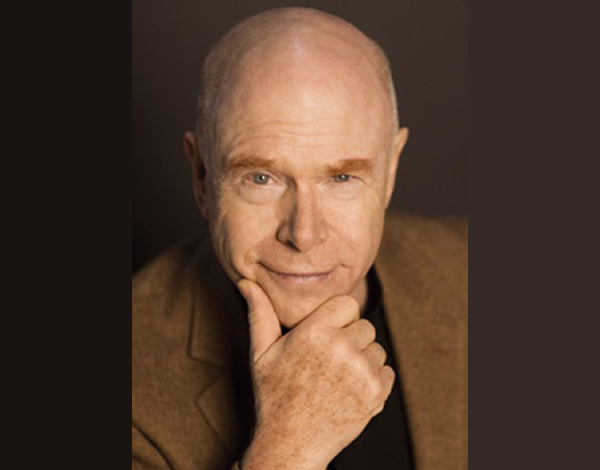
\includegraphics[trim={5cm 0 5cm 0},clip,width=.7\linewidth]{richard_rumelt.jpg}
		\caption{Richard Rumelt}
		\label{fig:rumelt}
	\end{center}
\end{marginfigure}

Üks põnevamaid tänapäevaseid arhitektuurimõtlejaid on Richard Rumelt\index{Rumelt, Richard}. Tema taust on inseneerias, seitsmekümnendatel osales ta kosmosesondi Voyager 1 konstrueerimisel. Tema ehk kuulsaim teos \enquote{Good strategy/bad strategy}\cite{rumelt2011good}. Raamatu allikaks on frustratsioon kuristikust srateegia ning tavaliselt strateegiaks nimetatu vahel\sidenote{Hea ülevaate tema seisukohtadest annab \url{https://www.youtube.com/watch?v=UZrTl16hZdk}}. Kui Steve Jobs\index{Jobs, Steve} 1997. aastal uuesti Apple juhiks sai, ei usutud tema edusse. Ometi suutis ta organisatsiooni mitte ainult päästa vaid ka ümber pöörata tehes asju, mida õpitakse ülikoolis esimesel kursusel. Ta loobus kõigest mittevajalikust keskendudes Apple äri tuumale. Rumelt ütleb, et keegi tegelikult ei oota, et keegi päriselt sel viisil strateegiaga tegeleb. Ehk, hea ja koherentne strateegia on haruldane ning üllatav.

Eespool kirjeldatud vaade strateegiale sisaldas sõnu nagu \enquote{turg} ja \enquote{konkurents} kehastades seega probleemi ökonomeetrilist aspekti. Kuigi kahtlemata õige, ei ole selline lähenemine kergesti rakendatav vabakonna, avaliku sektori ja näiteks koolide puhul ehk olukordades, kus turust ja teenustest rääkimine on keeruline\sidenote{Vt. pikemat arutelu \cite{rumelt1991strategic}}. Siia kuuluvad ka IT organisatisoonid, kes küll opereerivad ärilises keskkonnas kuid kelle tegevuse mõõdikud on harva puhtalt majanduslikud.

Rumelt pakubki alternatiivi sõnastades mitte strateegia definitsiooni vaid \enquote{hea} ja \enquote{halva} strateegia tunnused. 

Tema järgi on halb strateegia\index{Strateegia!Hea ja halb} selline:
\begin{description}
	\item[Keskendub eesmärkidele] Strateegia on tihti kombinatsioon toredatest asjadest ja asjadest, mida me tahaksime saavutada. Eesmärkide sõnastamine on kahtlemata oluline aga strateegia peaks ütlema ka midagi nende saavutamise kohta. Kui meie straeegia on \enquote{20\% kasumimarginaali ja 20\% käibekasvu aastas}, siis mida me siis ikkagi selle saavutamiseks teeme?
	\item[On pehme ja kohev] Selline strateegia on ebamäärane kasutades raskesti defineeritavaid mõisteid ja ebaselgeid kontseptsioone. \enquote{Oleme kliendikeskne innovatsiooniliider läbi tarneahela sünergia võimendamise} kõlab uhkesti aga strateegia ei saa olla otsuste aluseks ilma, et ta oleks üheselt ja selgelt arusaadav. 
	\item[Ei sisalda probleemi] Räägitakse asjadest, mida me loodame saada, rääkimata olukorrast, kus me oleme. Et kuhugi minema hakata, on oluline kokku leppida, kus parasjagu ollakse ja kuidas seda olukorda mõttestatakse. On oluline vahe, kas organisatsioon on \emph{ainult} või \emph{juba} kaheksakümneprotsendiline turuosa
	\item[Sarnaneb Tootsi peenrale] Selline strateegia sisaldab hirmpikka loetelu eri asjadest, millega organisatsioon peaks tegelema ning mida kõike saavutama. Paraku on suur osa olulisi eesmärke üksteist välistavad ning nii ei ütle selline strateegia midagi peale selle, et selle koostaja ei suuda valikuid teha
\end{description}

Hea strateegia tunnused pakub Rumelt välja järgmised:
\begin{description}
	\item[Tal on selge kolmeosaline tuum] Hea strateegia peab sisaldama diagnoosi (kuidas me mõttestame meie ees seisva probleemi\sidenote{Huvitaval kombel teeb Rumelt eelduse, et kõigil on probleemid. Et kõigil on keskne hulk jõude, milledele vastu seismine nõuab pingutust. On üsna keeruline ette kujutada, millised on need jõud näiteks Apple või Google puhul. Kahtlemata on neil väljakutseid kuid tõenäoliselt on raske välja tuua üht ja eksistentsiaalset.} tuuma), juhtpoliitikat (milles meie lahendus seisneb) ja koherentset tegevusplaani (millised sammud võetakse ette probleemi lahendamiseks)
	\item[Sisaldab saavutatavat eesmärki] Hea strateegia osa on miski, mida on võimalik teatud pingutusega usutavalt saavutada. See miski peab olema konkreetne ning suhteliselt lühikese ajahorisondiga. Selline eesmärk annab tegevusele suuna ning aitab hinnata progressi
	\item[Eeldab entroopiat ja inertsi] \index{Entroopia}Strateegia rakendamise puhul on kõige suuremaks raskuseks tõenäoliselt organisatsioon ise. Algne plaan muutub ajas ja organisatsiooni hierarhias liikudes järjest hägusamaks ja sellega tuleb arvestada. Samuti on alust eeldada, et muutused organisatsioonis vastuseisu tekitavad ning plaan peab seda peegeldama
\end{description}

\section{Strateegia kasutusest}
\label{sec:strateegia:kasutu}
Oma strateegia ajaloos osundab Freedman, et Lääne kultuuriruumis kerkis strateegia kui oluline kontseptsioon esile alles kaheksateistkümnendal sajandil seoses sõja kui sellise keerukuse kasvuga\cite{freedman2013strategy}. Ühest küljest tekkis arvamus, et sõda, nagu teisedki eluvaldkonnad võiks süsteemsest mõtlemisest kasu saada. Kuid teisalt muutus sõda oma massiarmeede ja logistika-ahelatega ühte peasse mahtumiseks liiga keeruliseks. Enam ei olnud võimalik strateegia formuleerimist ja ellu viimist mõistlikult ühendada. Ka äristrateegia esile kerkimist seostab ta ettevõtete praktilise vajadusega liikuda kvantitatiivselt kasvult kvalitatiivsele.

See, loomulikult, ei tähenda, et varasemalt kuidagi oskamatult sõditud või firmasid juhitud oleks. Puudus lihtsalt praktiline vajadus eraldiseisva strateegia kontseptsiooni järele. Piisas kas lihtsast õnnest või usust geniaalsesse sõjapealikkusse. Strateegia oli suuresti välja hääldamata ning juurtega kommetes ning tavades\sidenote{Keeley war before civilization via Freedman}

Siit tuleneb oluline järeldus: strateegiat ei ole alati vaja. Kuna töö on ressursi- ja ajamahukas (ning kasutu strateegia taustal võib kergesti rumalasse olukorda jääda), siis on oluline mõista, millal strateegiaga tegeleda ei ole mõtet.

Skype\index{Skype} varastel aastatel puudus ettevõttel strateegiadokument selle klassikalises mõttes. Ei toimunud ka eraldi strateegia arendamise protsessi. Ometi võis juhusliku kontoris kohatud inimese käest saada küsimusele \enquote{millega te siin tegeleme?} konkreetse ja ammendava vastuse. Ja need vastused langesid põhijoontes kokku. Kuidas nii? Meie ees toona seisnud probleem oli väga konkreetne ja üheselt arusaadav ka ilma suuri sõnu tegemata. Oli vaja ise ellu jäädes telekomiturg pikali lükata. Suhteliselt väikeses kitsa ringi inimeste ümber koondunud organisatsioonis on tegemist vajav selge ka ilma eksplitsiidse strateegiata. 

Piibel ütleb, et \enquote{võidujooks pole kiiretele ja lahing tugevatele}. Ja, tõesti, suure hulga ressursside igasugune enam-vähem mõistlik kasutamine viib reeglina soovitud tulemusele ka ilma suurema strateegiata. Võib kuluda vähem või rohkem aega või ressursse aga töö saab tehtud. Nagu insenerid vahel ütlevad: \enquote{Ei ole lahendamatuid probleeme, on liiga väikesed haamrid}. Kui paras haamer käepärast ei ole mõtet arutada, kas võtta ta paremasse või vasakusse kätte.

Kolmas põhjus strateegiat mitte omada on kontrolli puudumine. Isegi kui käsitleda strateegiat kui suure hulga isiklike strateegiate sünergeetilist summat, on strateegia kujundamiseks ikkagai vaja neid isiklikke lähenemisi suunata. Kontroll võib puududa kas ülemiste juhtimistasandite poolt seatud reeglite, alumiste tasandite vastuseisu või usalduskreedidi puudumise tõttu juhi vastu. Kuidas ka ei oleks, sellisel juhul strateegiaga tegelemine on kindel viis end lolliks teha. 

Kokkuvõttes, strateegiaga ei ole mõtet tegeleda kolmel juhul:
\begin{itemize}
	\item Kui ollakse väike ning keskendunud
	\item Kui ollakse suur ja tugev
	\item Kui olukorda ei kontrollita piisavalt
\end{itemize}

Tähelepanelik lugeja kindlasti märkab, et ükski toodutest ei ole selgepiiriline või ühene. Millal ollakse \enquote{suur ja tugev}? Lapsed ja organisatsioonid võivad ootamatult kiiresti kasvada, tänane tugevus võib homme olla nõrkus ning ka suurim juht võib end nurka mängida. On oluline järjepidavalt hinnata oma organisatsiooni ning selle vajadust strateegia järele. Nii tegelemine mitteproduktiivsete asjadega kui mittetoimivast strateegiast tulenev võlts kindlustunne võivad organisatsioonile hukatuslikuks osutuda. 

\section{IT ja äristrateegia}
\begin{itemize}
	\item Idee sellest, et sõjaväeline strateegia seisab eraldi tsiviilstrateegiast, tuleneb kontrollisoovist \cite{freedman2013strategy} [p 242.]. Sealsamas kontroll sõjavälja üle läbi vaenlase hävitamise
	\item Põhjuslikkus ja õppiv vs. kontrolliv organisatsioon \cite{senge19905th}
	\item Liivakella väärtusmudel \cite{hing}.\cite{barrett2013liberating} Õppiv organisatsioon ja ühine strateegia mõlemad eeldavad seega teatud väärtusmudeli olemasolu organisatsioonis. Ilma 4. tasandi väärtusteta on jube keeruline koostööd teha või õppivat organisatsiooni ehitada. 
	\item Viide QA sektsiooni, Kaizen on hea õppiva organisatsiooni näide.
\end{itemize}

\section{Strateegia kui kommunikatsioon}
Strateegi anne seisneb tema võimes kommunikeerida oma inisighti olukorra kohta ning selle järelmeid tegevuse mõttes. Ei ole üks-üheselt seotud arusaama õigsusega, kuid mingi piirini on seos olemas: täitsa paikapidamatut mõtet on raske müüa kuid väga hästi võib olla müüdav vale kuid meeldiv arusaam asjadest.

\section{Küsimusi aruteluks}
\subsection{Kuidas lahutada IT strateegia äristrateegiast?}
\label{sec:strategy:q1}
Kui meie loengute kandev teema on \enquote{Infotehnoloogia strateegiline juhtimine} tundub sellest järelduvat, et on võimalik tegeleda IT strateegia kui millegi äristrateegiast eraldi seisvaga. Samas on ilmselt selge, et IT ei saa toimida ärist eraldi ning seosed peavad olema tugevad.

Kindlasti ei ole mõtet rääkida IT strateegiast juhtudel, kui strateegiat kui sellist üldse vaja pole \sidenote{Vt. lõik \nameref{sec:strateegia:kasutu}}. IT kontekstis on tüüpiliselt põhjuseks liig range korporatiivne keskkond, mis ühtlustab IT organisatsioonis kõik alates personalipoliitikast (tasustamine, värbamine, tulemuste hindamine jne.) kuni operatiivmudelini (osta/ehita otsused, lepingulised suhted, mõõdikud jne.). Sel juhul võib ja peab IT-juht küll vastutama kõigi strateegiliste valdkondade toimimise eest kuid saab seda teha vaid rangelt etteantud piirides muutudes strateegist strateegia koostajast selle elluviijaks.

Siit järeldub, et IT juhile on oma strateegia ellu viimiseks hädavajalik olla juhtkonnale tõsiseltvõetav partner. Vaid nii õnnestub kaasa rääkida äristrateegia kujundamisel ning saavutada vabadus toimetada IT strateegiaga. 

IT ja äristrateegia seoseid saab mõtestada näiteks kasutades Rumelti hea strateegia tunnuseid (vt.\nameref{sec:strategy:goodbad}). Hea IT strateegia peaks
\begin{description}
	\item[Omama probleemi, leitmotiivi ja tegevusplaani]. Probleemi sõnastamiseks tuleb aluseks võtta tuumprobleem äristrateegiast\sidenote{Selle puudumisel on mõistlik sõnastada probleem, mille taha on IT organisatsioon nõus koonduma. Vt. ka \ref{sec:strategy:q3}}. Seos ei saa olla aga automaatne. Kui äri probleemiks on liig kõrged kulud võib IT oma probleemi sõnasta nii läbi kulude kui ka näiteks informatsiooni kogumise ja kättesaaavaks tegemise. Kuidas ikkagi juhtus, et meie kulud kasvasid? Kui äri juhtiv poliitika on piisavalt üldine (\enquote{Jaga ja valitse}), sobib see ka ITle. Spetsiifilisematel juhtudel tuleb ilmselt sõnastada valdkonnaspetsiifiline lähenemine. IT tegevusplaani iga samm peaks olema seotud äristrateegia tegevusplaaniga
	\item[Sisaldama saavutatavat eesmärki] Nagu ka tegevusplaani puhul peaks IT eesmärk toetama organisatsiooni üldise eesmärgi saavutamist. Samas peab eesmärk olema ka tehnoloogilises plaanis saavutatav IT-juhi kontrolli all olevate vahendite abil. Tasub mõelda süsteemi piiride\index{Süsteem!Piirid} probleemist (vt. \nameref{sec:boundary})
	\item[Eeldama entroopiat ja inertsi] Nagu ka organisatsiooni oma, peab IT strateegia arvestama muutustega. Seda nii eesmärkide saavutatavuse kui tegevuskava mõttes. IT kontekstis võib siinkohal mõelda ka riskide juhtimisest kuid mitte ainult. IT on olemuslikult eesliinitööle lähemal (ja omab tugevamat tehnilist kompetentsi) ja võib näha inertsi seal, kus äri tasemel on lihtne muutus. Näiteks võib andmebaasiplatvormi vahetus ka tehnikule suhteliselt lihtsana tunduda kuni kellelegi ei meenu, et miskipärast on kunagi otsustatud massiivses koodibaasis läbivalt kasutada vanale platvormile spetsiifilisi lahendusi. Sel juhul on ülioluline, et äristrateegia muudetud saaks
\end{description}

\subsection{Kui kiiresti sumbuvad muutused organisatsioonis?}
\index{Muutused}
Ehk, \enquote{Kas äristrateegia muutus võib muuta majutus-strateegiat?}. Organisatsiooni kihilises mudelis (vt. joonis \ref{fig:stack}) on kõik kihid omavahel seotud. Muutus ühes põhjustab muutusi järgmistes. Seega tekib tahes tahmata küsimus sellest, kui kiiresti sellised muutused organisatsioonis sumbuvad. Ühest küljest võib IT tegeleda vaid tellija soovide täitmisega kuid teisalt võib ta ka investeerida paindlikku taristusse, mis sisuliselt ärist ei sõltu. Smauti sõltub vastus küsimusele olulisel määral muutuse olemusest.

\begin{marginfigure}
	\begin{center}
		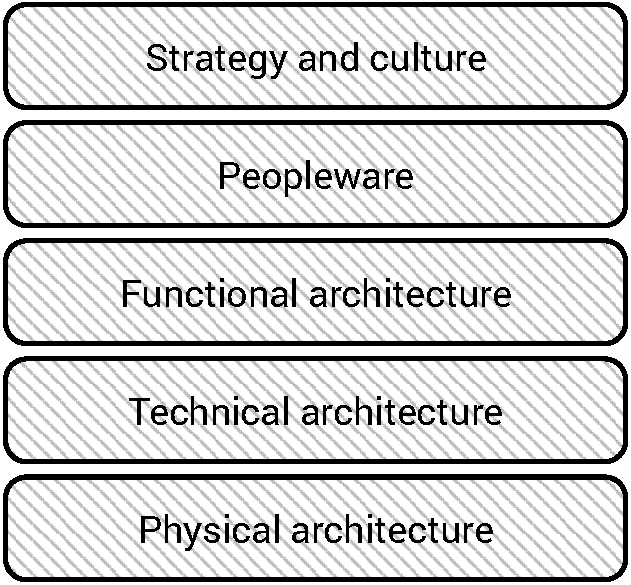
\includegraphics[width=\linewidth]{stack.pdf}
		\caption{Organisatsiooni kihiline mudel}
		\label{fig:stack}
	\end{center}
\end{marginfigure}

Peamine sõnum auditooriumist: tuleb leida tasakaal lihtsa käsutäitmise ning täiesti paindliku lahenduse vahel, kumbki ei ole soovitav.

\TODO vajab viidet N juhtumile ja stacki põhjalikku lahtikirjutust koos arutluskäiguga

\subsection{Kuidas juhtida mõistlikult ITd kui organisatsioon kui tervik ei ole mõistlikult juhitud?}
\label{sec:strategy:q3}
Elu näitab, et organisatsioone võib pikalt juhtida viisil, mida kindlasti mõistlikuks pidada ei saa. Kindlasti võib äriettevõtete langus kesta aastaid ning ka avalikus sektoris võivad demokraatlikud mehhanismid tekitada olukorra, mis tingimata juhtimislikult mõistlik ei ole. Seega tekib küsimus, kas ja kuidas mittemõistlikus organisatsioonis on võimalik tegeleda mõistliku IT juhtimisega.

Peamine sõnum auditooriumist: proovime pakkuda paremaid lahendusi (mõisnik ja banaan), seletame otsuste mõju (ajahorisondi küsimus).

Ei ole mõistlik organisatsiooni parandada läbi korraliku IT, nii liputab saba koera. Mõistlikum on aktepteerida, mida muuta ei saa (serenity prayer)
\ref{sec:strategy:q1}
\TODO korralikult lahti kirjutada
